\documentclass{article}
\usepackage{style-notes}

\newcounter{lecnum} 	% define counter for lecture number
\renewcommand{\thepage}{\thelecnum-\arabic{page}}	% define how page number is displayed (< lecture number > - < page number >)

% define lecture header and page numbers
% NOTE: to call use \lecture{< Lecture # >, < Lecture name >, < Chapter # >, < Chapter name >, < Section #s >}
\newcommand{\lecture}[5]{

    % define headers for first page
    \thispagestyle{empty} % removes page number from page where call is made

    \setcounter{lecnum}{#1}		% set lecture counter to argument specified

    % define header box
    \begin{center}
    \framebox{
      \vbox{\vspace{2mm}
    \hbox to 6.28in {\textbf{MATH 320: Probability} \hfill}
       \vspace{4mm}
       \hbox to 6.28in {{\hfill \Large{Lecture #1: #2} \hfill}}
       \vspace{2mm}
       \hbox to 6.28in {}%\hfill Chapters #3: #4 \small{(#5)}}
      \vspace{2mm}}
    }
    \end{center}
    \vspace{4mm}
    
    % define headers for subsequent pages
    \fancyhead[LE]{\textit{#2} \hfill \thepage} 		% set left header for even pages
    \fancyhead[RO]{\hfill \thepage}		% set right header for odd pages
}

% define macros (/shortcuts)
\newcommand{\bu}[1]{\textbf{\ul{#1}}}	% shortcut bold and underline text in one command


\begin{document}

\lecture{0}{Course Overview}{}{}{}

\bu{Big picture}\bigskip

Relationship between Probability and Statistics\bigskip
\begin{itemize}
    \item In a probability problem, the properties of the population are assumed known, and we use these to infer properties of the sample.
    \begin{figure}[H]
        \center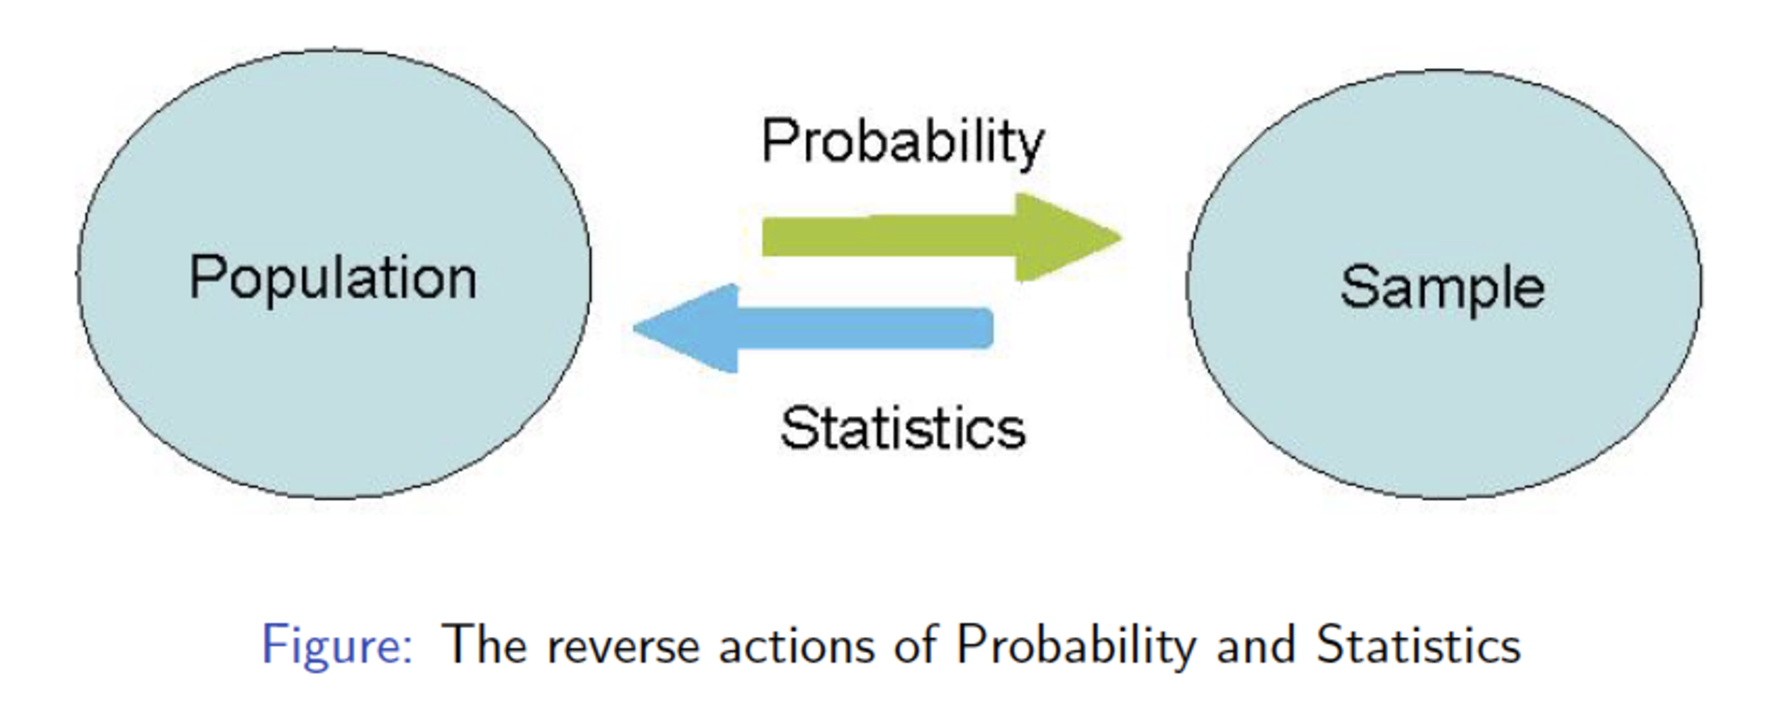
\includegraphics[scale=0.25]{test-1/probability-vs-statistics}
    \end{figure}\bigskip
    \item Whereas statistics is concerned with learning (inferring) population properties from sample information (which is the opposite of probability).
    \item Example:
    \begin{itemize}
        \item Suppose we know 75\% of batteries last longer than 1500 hours. $\rightarrow$
        \item[] We want to know the chance all 10 batteries in a pack last 1500 hours. $\rightarrow$\bigskip
        \item Suppose that out of 10 batteries, 6 are found to last more than 1500 hours. $\rightarrow$
        \item[] We want to know if that is enough evidence to conclude that the proportion of all batteries that last more than 1500 hours is less than 75\%. $\rightarrow$
    \end{itemize}\bigskip
    \item In spite of this difference, statistical inference itself would not be possible without probability because it is based on probability calculations.
\end{itemize}

\newpage

Courses you will take\bigskip
\begin{itemize}
    \item MATH 320 Probability (Fall)
    \begin{itemize}
        \item This deals with the building blocks of inferential statistics, which is probability.
        \item Calculating probabilities: Set theory, counting, probabilities of events, random variables
        \item Univariate distributions: Random variables / distributions, probabilities of events, summaries of random variables, applications
        \item Multivariate distributions: Repeat above, now with more than one random variable.
    \end{itemize}\bigskip
    \item MATH 321 Mathematical Statistics (Spring)
    \begin{itemize}
        \item This deals with theory and practice of statistics $\rightarrow$ We have data, now what do we do with it?
        \item Descriptive statistics: Summarizing a whole data set with a single or a few measures (e.g. mean, standard deviation, minimum) and visualizing datasets (e.g. histograms, boxplot).
        \item Inferential statistics: Collecting data, analyzing it, and making inferences on parameters using probability concepts.
    \end{itemize}
\end{itemize}\bigskip

\vspace{15pt}

\bu{Exam P syllabus}

\begin{figure}[H]
    \center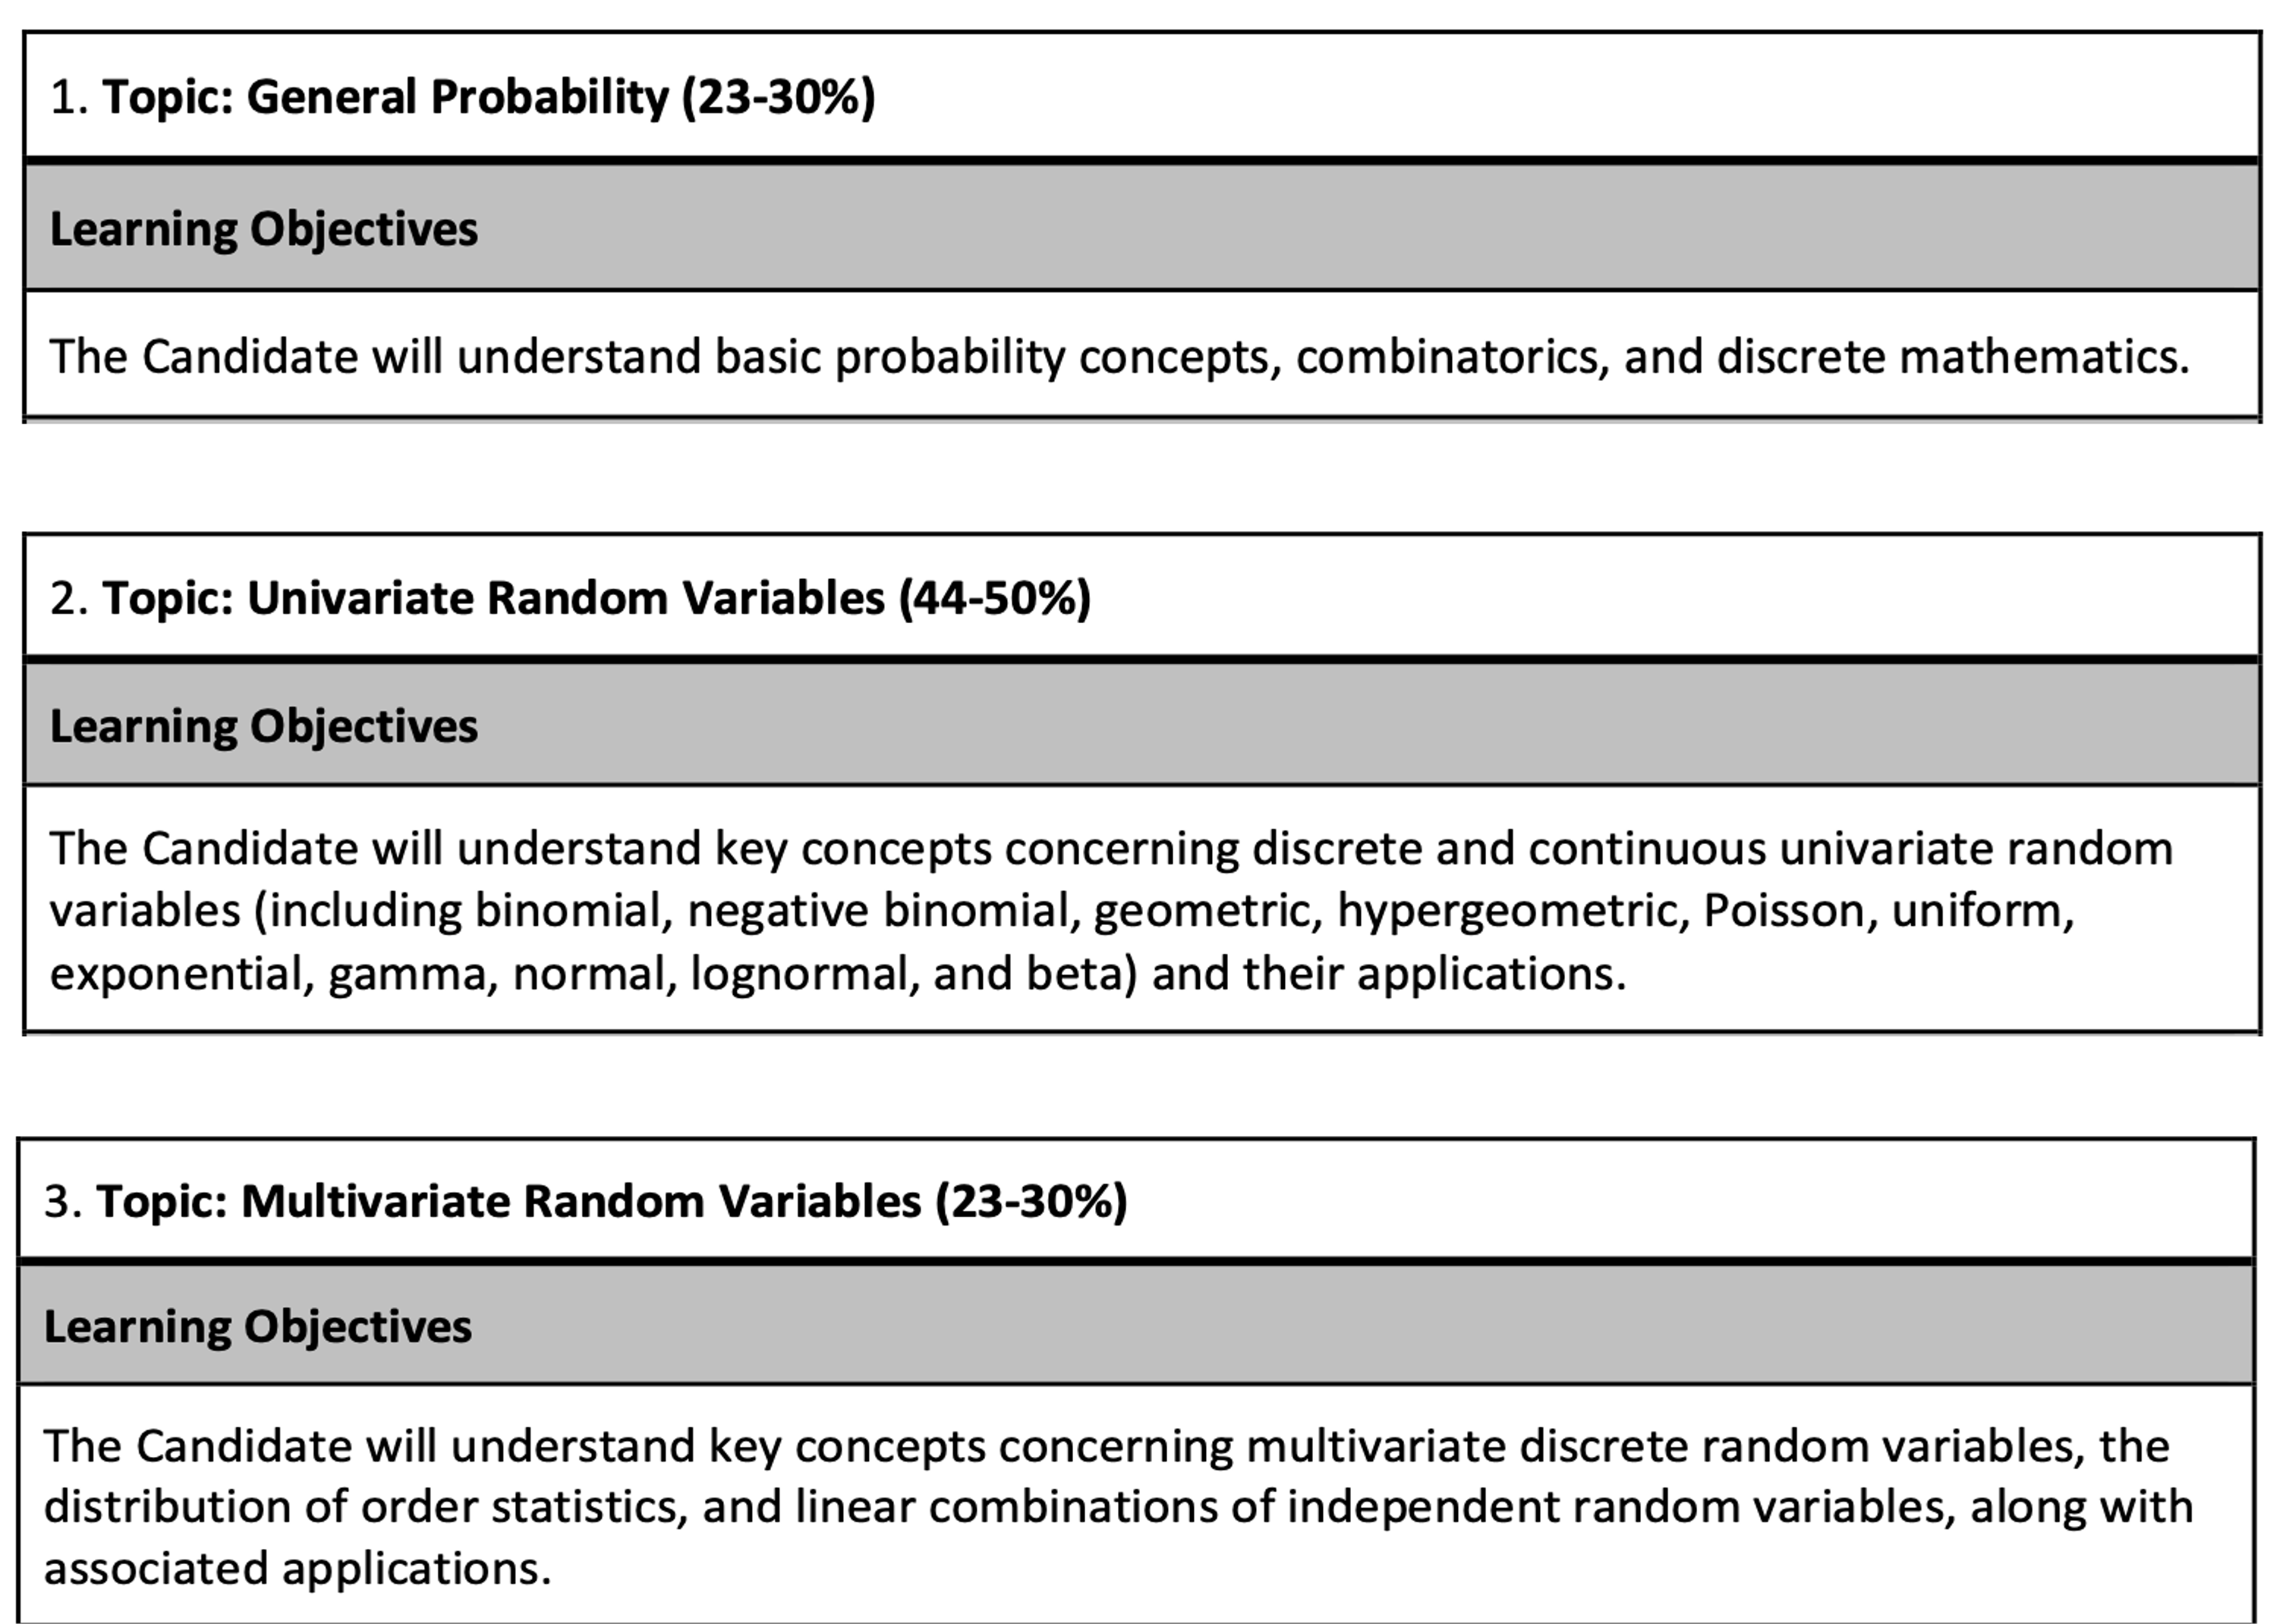
\includegraphics[scale=0.5]{test-1/exam-p-syllabus}
\end{figure}

\end{document}